\documentclass[main.tex]{subfiles}
% 函数的微分和导数
\begin{document}
%======================================
\subsection{一元函数的导数与微分(回顾)}
我们在本科的高等数学课上已经学过一元函数的导数与微分。我们复述它们,一是为了明确符号的记法,二是为了与后面介绍的多维的情况作对比。

回顾高阶无穷小定义,简述为:若函数$f\left(x\right)$在点$x_0$处有极限$\lim_{x\to x_0}f\left(x\right)=0$,则称函数$f\left(x\right)$是当$x\to x_0$时的一个无穷小。若函数$f\left(x\right),g\left(x\right)$是当$x\to x_0$时的无穷小,且$\lim_{x\to x_0}f\left(x\right)/g\left(x\right)=0$,则称$f\left(x\right)$是当$x\to x_0$时$g\left(x\right)$的一个高阶无穷小。

\begin{definition}[一元函数的导数]\label{def:II.4.7}\cite[定义2.1.1]{华工高数2009上}
    设函数$y=f\left(x\right)$在点$x_0$的某个邻域内有定义,当自变量$x$在点$x_0$处取得改变量$\Delta x$,且点$x_0+\Delta x$在上述邻域内时,相应地,函数的改变量为
    \[
        \Delta y=f\left(x_0+\Delta x\right)-f\left(x_0\right)\text{,}
    \]
    如果极限
    \[
        \lim_{\Delta x\to 0}\frac{\Delta y}{\Delta x}=\lim_{\Delta x\to 0}\frac{f\left(x_0+\Delta x\right)-f\left(x_0\right)}{\Delta x}
    \]
    存在,称函数$f\left(x\right)$在点$x_0$处\emph{可导}(或\emph{存在导数}),上述极限值称为\emph{函数$f$在点$x_0$处的导数},记为
    \[f^\prime\left(x_0\right),\quad\left.y^\prime\right|_{x=x_0},\quad\left.\frac{df}{dx}\right|_{x=x_0},\quad\text{或}\left.\frac{dy}{dx}\right|_{x=x_0},
    \]
    即
    \[
        f^\prime\left(x_0\right)=\lim_{\Delta x\to 0}\frac{f\left(x_0+\Delta x\right)-f\left(x_0\right)}{\Delta x}\text{。}
    \]
    若该极限不存在,称\emph{函数$f\left(x\right)$在$x_0$处不可导}。
\end{definition}

\begin{definition}[一元函数的微分]\label{def:II.4.8}\cite[定义2.5.1]{华工高数2009上}
    设函数$y=f\left(x\right)$在点$x_0$的某邻域内有定义,当$x$在点$x_0$处获得增量$\Delta x$时,如果相应的函数增量$\Delta y=f\left(x_0+\Delta x\right)-f\left(x_0\right)$可以表示为
    \[\Delta y=A\Delta x+o\left(\Delta x\right)\text{,}
    \]
    其中,常数$A$与$\Delta x$无关(仅与$x_0$有关),而$o\left(\Delta x\right)$是较$\Delta x\left(\Delta x\to 0\right)$的高阶无穷小,则称函数$y=f\left(x\right)$\emph{在点$x_0$处可微(differentiable at $x_0$)}。且称$A\Delta x$为函数$y=f\left(x\right)$在点$x_0$处对应于自变量增量$\Delta x$的\emph{微分(differential of $y=f\left(x\right)$ at $x_0$)},记作$dy$,即
    \[
        dy=A\Delta x\text{,}
    \]
    也常把$A\Delta x\left(A\neq 0\right)$称为函数增量$\Delta y$的\emph{线性主部}。
\end{definition}

在$\Delta y$的分解式中,由于其值主要取决于线性主部$A\Delta x$,因此当$\Delta x\to 0$时,我们可以写
\[
    \Delta y\approx dy=A\Delta x\text{。}
\]

\begin{theorem}\label{thm:II.4.5}\cite[定理2.5.1]{华工高数2009上}
    函数$y=f\left(x\right)$在点$x_0$处可微的充分必要条件是:函数$y=f\left(x\right)$在点$x_0$处可导,且当$y=f\left(x\right)$在点$x_0$处可微时,其微分是
    \[
        dy=f^\prime\left(x_0\right)\Delta x\text{。}
    \]
\end{theorem}
\begin{proof}
    略\cite[p.~103]{华工高数2009上}。
\end{proof}

关于符号“d”的意义,这里给出一个比高等数学课本\cite[p.~104]{华工高数2009上}更仔细的说明。

由函数微分的定义可知,函数$f\left(x\right)$在点$x_0$处对应于自变量增量$\Delta x$的微分$dy=f'\left(x_0\right)\Delta x$,实际上是一个由点$x_0$引出的函数,记为$df_{x_0}:\mathbb{R}\rightarrow\mathbb{R},df_{x_0}\left(x\right)=f'\left(x_0\right)x,\forall x\in I$,其中区域$I$是所有满足$x_0+x$在函数可微的$x_0$的邻域的所有实数$x$的集合。

若视$x$本身为一个恒等映射,即$x\left(p\right)=p,\forall p\in\mathbb{R}$,则函数$x$在点$p$处的微分也是一个由点$p$引出的函数,且$dx_p\left(u\right)=x^\prime\left(p\right) u=1\times u,\forall u\in\mathbb{R}$,也是一个恒等映射。同时我们看到,函数$dx_p\left(u\right)$是$u\to 0$的无穷小。

考虑复合映射$f\left(x\left(p\right)\right)$在点$p_0$处的微分,它是由点$p_0$引出的函数,\[d\left(f\circ x\right)_{p_0}\left(u\right)=\left.\frac{d\left(f\circ x\right)}{dp}\right|_{p=p_0}u=f^\prime\left(x(p_0\right))x^\prime\left(p_0\right)u=f^\prime\left(p_0\right)dx_{p_0}\left(u\right)\]
而且函数$d\left(f\circ x\right)_{p_0}\left(u\right)$与$dx_{p_0}\left(u\right)$是$u\to 0$时的同阶无穷小,$f^\prime\left(p_0\right)$就是这两个无穷小的比值,该结论对所有$p_0,u\in\mathbb{R}$都成立,因此若去掉$p_0$和$u$简记:
\[df\left(x\right)=f^\prime dx\]
则
\[f^\prime=\frac{df}{dx}\text{。}\]
因此,当我们把导数当作分数来处理时,实际是在上述的意义上视导数为两个微分作为同阶无穷小的比值。

\begin{definition}[一元向量函数的导数]\label{def:II.4.9}
    设函数$\mathbf{f}:\mathbb{R}\supset D\rightarrow\mathbb{R}^n$的极限
    \[
        \lim_{h\to 0}\frac{\mathbf{f}\left(t+h\right)-\mathbf{f}\left(t\right)}{h}
    \]
    存在,则称函数$\mathbf{f}\left(x\right)$在$x=t$处\emph{可导}。该极限是\emph{函数$\mathbf{f}\left(x\right)$在$x=t$处的导数},记为
    \[
        \left.\frac{d\mathbf{f}\left(x\right)}{dx}\right|_{x=t}\equiv\lim_{h\to 0}\frac{\mathbf{f}\left(t+h\right)-\mathbf{f}\left(t\right)}{h}
    \]
\end{definition}

由一元\emph{标量}函数求导的法则可证有以下一元\emph{向量}函数求导法则:对任意函数$\mathbf{f}:\mathbb{R}\supset D\rightarrow\mathbb{R}^n,\mathbf{g}:D\rightarrow\mathbb{R}^n$,
\begin{itemize}
    \item $\frac{d\mathbf{c}}{dt}=0,\mathbf{c}\in\mathbb{R}^n$是常向量
    \item $\frac{d}{dt}\left(\alpha\mathbf{f}+\beta\mathbf{g}\right)=\alpha\frac{d}{dt}\mathbf{f}+\beta\frac{d}{dt}\mathbf{g},\forall \alpha,\beta\in\mathbb{R}$
    \item $\frac{d}{dt}\left[u\left(t\right)\mathbf{f}\left(t\right)\right]=\frac{du}{dt}\mathbf{f}+u\frac{d}{dt}\mathbf{f},\forall u:D\rightarrow\mathbb{R}$
    \item $\frac{d}{dt}\left(\mathbf{f}\cdot\mathbf{g}\right)=\frac{d\mathbf{f}}{dt}\cdot\mathbf{g}+\mathbf{f}\cdot\frac{d\mathbf{g}}{dt}$
    \item $\frac{d}{dt}\left(\mathbf{f}\times\mathbf{g}\right)=\frac{d\mathbf{f}}{dt}\times\mathbf{g}+\mathbf{f}\times\frac{d\mathbf{g}}{dt}$
\end{itemize}

\begin{definition}[多元标量值函数的偏导数]\label{def:II.4.10}
    给定函数$f:\mathbb{R}^n\supset D\rightarrow\mathbb{R}$,若对某一$i\in\left\{1,\cdots,n\right\}$,极限
    \[
        \lim_{t\to0}\frac{f\left(\cdots,x_{i}+h,\cdots\right)-f\left(\cdots,x_{i},\cdots\right)}{t}
    \]
    当$x_i=x_{i0}$时存在,则称该极限为\emph{函数$f\left(\mathbf{x}\right)$对第$i$个变量$x_i$在$x_i=x_{i0}$处的的偏导数(partial derivative)},记为
    \[\left.\frac{\partial f\left(\mathbf{x}\right)}{\partial x_i}\right|_{x_i=x_{i0}}\equiv\lim_{t\to0}\frac{f\left(\cdots,x_{i}+h,\cdots\right)-f\left(\cdots,x_i,\cdots\right)}{t}
    \]
\end{definition}

\begin{theorem}\label{thm:II.4.6}\footnote{即高等数学\cite[p.~16]{华工高数2009下}定理7.2.1向$n$维的推广。}
    如果函数$f:\mathbb{R}^n\rightarrow\mathbb{R}$的一个二阶混合偏导数$\frac{\partial^2f}{\partial x_i\partial x_j}$在$\mathbb{R}^2$的一个开子集$S$上处处连续,则二阶混合偏导数$\frac{\partial^2f}{\partial x_j\partial x_i}$在$S$上处处存在,且$\frac{\partial^2f}{\partial x_i\partial x_j}=\frac{\partial^2f}{\partial x_j\partial x_i}$。
\end{theorem}
\begin{proof}
    略\footnote{进一步了解:\href{https://en.wikipedia.org/wiki/Symmetry_of_second_derivatives}{Symmetry of second derivatives}。}
\end{proof}

\begin{definition}[向量函数的偏导数]\label{def:II.4.11}
    函数$\mathbf{f}:\mathbb{R}^n\supset D\rightarrow\mathbb{R}^m$对第$i$个变量在$x_i=x_{i0}$处的\emph{偏导数}定义如下向量
    \[
        \left.\frac{\partial \mathbf{f}\left(\mathbf{x}\right)}{\partial x_i}\right|_{x_i=x_{i0}}\equiv\left(\begin{array}{c}
                \left.\frac{\partial f_1\left(\mathbf{x}\right)}{\partial x_i}\right|_{x_i=x_{i0}} \\
                \vdots                                                                             \\
                \left.\frac{\partial f_m\left(\mathbf{x}\right)}{\partial x_i}\right|_{x_i=x_{i0}}\end{array}\right)\in\mathbb{R}^m
    \]
    其中,$\mathbf{x}=\left(x_1,\cdots,x_n\right)^\intercal\in\mathbb{R}^n$。
\end{definition}


%==========================================
\subsection{向量函数的微分和导数}
回顾多元标量函数的全微分的定义\cite[“定义7.3.1”,p.~19]{华工高数2009下}——

\begin{definition}[多元标量值函数的微分]\label{def:II.4.12}
    若函数$z=f\left(x,y\right)$在点$P_0\left(x_0,y_0\right)$的全增量
    \[
        \Delta z=f\left(x_0+\Delta x,y_0+\Delta y\right)-f\left(x_0,y_0\right)
    \]
    可表示为
    \[
        \Delta z=A \Delta x+ B \Delta y+o\left(\rho\right)
    \]
    其中$A,B$只与点$\left(x_0,y_0\right)$有关,而与$\Delta x,\Delta y$无关。又$\rho=\sqrt{\left(\Delta x\right)^2+\left(\Delta y\right)^2}$,$o\left(\rho\right)$是当$\rho\rightarrow 0$时$\rho$的高阶无穷小,则称函数$z=f\left(x,y\right)$在点$P_0\left(x_0,y_0\right)$可微分,且把$\Delta z$的线性主部$A\Delta x+B\Delta y$称为\emph{函数$z=f\left(x,y\right)$在点$P_0\left(x_0,y_0\right)$的全微分(differential)},记作
    \[
        \left.dz\right|_{x=x_0,y=y_0}=A\Delta x+B\Delta y\text{或}df\left(x_0,y_0\right)=A\Delta x+B\Delta y
    \]
    如果函数$z=f\left(x,y\right)$在区域$D$内每一点都可微,则称这函数\emph{在$D$内可微(differentiable in $D$)}。
\end{definition}

如果函数$z=f\left(x,y\right)$在点$P_0\left(x_0,y_0\right)$处可微,则有
\begin{align*}
                    & f\left(x_0+\Delta x,y_0+\Delta y\right)-f\left(x_0,y_0\right)=A\Delta x+B\Delta y+o\left(\rho\right)                                                 \\
    \Leftrightarrow & o\left(\rho\right)=f\left(x_0+\Delta x,y_0+\Delta y\right)-f\left(x_0,y_0\right)-\left(A\Delta x+B\Delta y\right)                                    \\
    \Leftrightarrow & \lim_{\rho\to0}\frac{f\left(x_0+\Delta x,y_0+\Delta y\right)-f\left(x_0,y_0\right)-\left(A\Delta x+B\Delta y\right)}{\sqrt{\Delta x^2+\Delta y^2}}=0 \\
    \Leftrightarrow & \lim_{\rho\to0}\frac{\Delta z-dz}{\rho}=0
\end{align*}
其中$\rho=\sqrt{\Delta x^2+\Delta y^2}$。上面的极限式是定义\ref{def:II.4.12}的等价定义式。我们其实可以不引入某个高阶无穷小$o\left(\rho\right)$,直接用使该极限式成立的$A,B$的存在性来定义函数的可微性。下面我们按照把函数微分的定义推广到一般的向量函数。

\begin{definition}[向量值函数的微分]\label{def:II.4.13}
    若函数$\mathbf{f}:\mathbb{R}^n\supset D\rightarrow\mathbb{R}^m$在其定义域内某点$\mathbf{x}_0\in D$处,存在一个线性变换$\mathbf{L}:\mathbb{R}^n\rightarrow\mathbb{R}^m$使得对任意$\mathbf{x}_0$的邻域$N\left(\mathbf{x}_0\right)$中的点$\mathbf{x}\in N\left(\mathbf{x}_0\right)$,
    \[\lim_{\mathbf{x}\rightarrow\mathbf{x}_0}\frac{\mathbf{f}\left(\mathbf{x}\right)-\mathbf{f}\left(\mathbf{x}_0\right)-\mathbf{L}\left(\mathbf{x}-\mathbf{x}_0\right)}{\left\|\mathbf{x}-\mathbf{x}_0\right\|}=\mathbf{0}\]
    就称\emph{函数$\mathbf{f}\left(\mathbf{x}\right)$在$\mathbf{x}_0$处可微分(differentiable at $\mathbf{x}_0$)}。向量$\mathrm{d}_{\mathbf{x}=\mathbf{x}_0}\mathbf{f}\left(\mathbf{x}\right)\equiv\mathbf{Lx}-\mathbf{Lx}_0$,称\emph{函数$\mathbf{f}\left(\mathbf{x}\right)$在$\mathbf{x}_0$处的微分(the differential of $\mathbf{f}\left(\mathbf{x}\right)$ at $\mathbf{x}_0$)}。如果函数$\mathbf{f}\left(\mathbf{x}\right)$在开集$S\subseteq D$内的每一点上都可微分,则称函数是\emph{$S$上的可微函数(differentiable function on $S$)}。
\end{definition}

我们可以根据向量函数的定义来看出,定义\ref{def:II.4.13}就是定义\ref{def:II.4.12}的推广。延用定义\ref{def:II.4.13}的设定,设$\mathbf{f}=\left(f_1,\cdots,f_m\right)^\intercal$,$\mathbf{x}=\left(x_1,\cdots,x_n\right)^\intercal$,$\mathbf{x}_0=\left(x_{01},\cdots,x_{0n}\right)^\intercal$,则函数$\mathbf{f}\left(\mathbf{x}\right)$在$\mathbf{x}_0$处的全增量是:
\[
    \mathbf{f}\left(\mathbf{x}\right)-\mathbf{f}\left(\mathbf{x}_0\right)=\left(
    \begin{array}{c}
            f_1\left(x_1,\cdots,x_n\right)-f_1\left(x_{01},\cdots,x_{0n}\right) \\
            \vdots                                                              \\
            f_m\left(x_1,\cdots,x_n\right)-f_m\left(x_{01},\cdots,x_{0n}\right)
        \end{array}\right)
\]
可见我们实际考虑的是$m$个$n$元标量值函数分别在点$x_{01},\cdots,x_{0n}$处的全增量。如果在这些点上这些标量值函数分别都可微,则$\mathbf{f}$的每个坐标函数的全增量都可按定义\ref{def:II.4.12}写成
\[
    f_i\left(x_1,\cdots,x_n\right)-f_i\left(x_{01},\cdots,x_{0n}\right)=\sum_{j=1}^n L_{ji}\left(x_j-x_{0j}\right)+o\left(\rho\right),i=1,\cdots,m
\]
其中,$L_{ij}$是“线性主部”的系数,只与$\left(x_{01},\cdots,x_{0n}\right)$有关,$\rho=\left(\sum_{j=1}^n\left(x_j-x_{0j}\right)^2\right)^{1/2}=\left\|\mathbf{x}-\mathbf{x}_0\right\|$,$o\left(\rho\right)$是当$\rho\to 0$时$\rho$的高阶无穷小。这等价于如下极限式
\[
    \lim_{\rho\to 0}\frac{1}{\left\|\mathbf{x}-\mathbf{x}_0\right\|}\left(\begin{array}{c}
            f_1\left(x_1,\cdots,x_n\right)-f_1\left(x_{01},\cdots,x_{0n}\right)-\sum_{j-1}^nL_{1j}\left(x_j-x_{0j}\right) \\
            \vdots                                                                                                        \\
            f_m\left(x_1,\cdots,x_n\right)-f_m\left(x_{01},\cdots,x_{0n}\right)-\sum_{j-1}^nL_{mj}\left(x_j-x_{0j}\right)
        \end{array}\right)=\left(\begin{array}{c}0\\\vdots\\0\end{array}\right)
\]
若线性变换$\mathbf{L}$在标准基下的矩阵坐标就是$L_{ij}$,则上式等价于定义\ref{def:II.4.13}的极限式。

我们以一个易于作图的例子说明函数微分的几何意义。函数$f:\mathbb{R}^2\rightarrow\mathbb{R}$的图像是3维欧几里得空间中的一个曲面(如图\ref{fig:II.4.7})。$f$在点$\mathbf{x}_0$处的微分$\left(\mathrm{d}_{\mathbf{x}=\mathbf{x}_0}f\left(\mathbf{x}\right)\right)\left(\mathbf{x}-\mathbf{x}_0\right)$定义了该曲面在$\mathbf{x}=\mathbf{x}_0$处的切平面。随着$\mathbf{x}$接近$\mathbf{x}_0$,函数$f$的全增量$f\left(\mathbf{x}\right)-f\left(\mathbf{x}_0\right)$将比$\mathbf{x}$接近$\mathbf{x}_0$更快地接近切平面。

\begin{figure}[h]
    \centering
    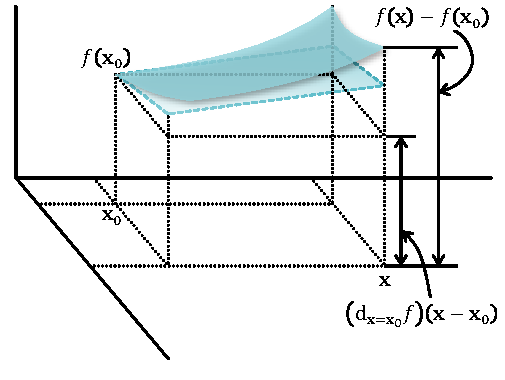
\includegraphics[width=0.75\textwidth]{images/II.4.7.pdf}
    \caption{向量函数的极限(定义\ref{def:II.4.5})的图像化理解。}
    \label{fig:II.4.7}
\end{figure}

我们接下来考察函数可微与可导的关系,即函数可微的充分和必要条件\footnote{这部分内容可以与本科高等数学课上的相应内容对比学习,特别是关于必要非充份条件和充份非必要条件的例子(“二、全微分存在的条件”\cite[p.~20]{华工高数2009下}。)}。首先,以下定理是函数在某点处可微分的必要条件,它同时也给出了$\mathbf{L}$或其坐标矩阵$L_{ij}$的计算方法。

\begin{theorem}\label{thm:II.4.7}
    设函数$\mathbf{f}:\mathbb{R}^n\supset D\rightarrow\mathbb{R}^m$在点$\mathbf{x}_0\in D$处可微分,即存在线性变换$\mathbf{L}\in\mathcal{L}\left(\mathbb{R}^n,\mathbb{R}^m\right)$满足
    \[
        \lim_{\Delta\mathbf{x}\to\mathbf{0}}\frac{\mathbf{f}\left(\mathbf{x}_0+\Delta \mathbf{x}\right)-\mathbf{f}\left(\mathbf{x}_0\right)-\mathbf{L}\Delta\mathbf{x}}{\left\|\Delta\mathbf{x}\right\|}=\mathbf{0}
    \]
    则$\mathbf{f}$的每个坐标函数在$\mathbf{x}_0$处的每个偏导数
    \[
        \left.\frac{f_i\left(\mathbf{x}\right)}{\partial x_j}\right|_{\mathbf{x}=\mathbf{x}_0},i=1,\cdots,m,j=1,\cdots,n
    \]
    都存在。若$\left\{\mathbf{\hat{e}}_1,\cdots\mathbf{\hat{e}}_n\right\},\left\{\mathbf{\hat{u}}_1,\cdots,\mathbf{\hat{u}}_m\right\}$分别是$\mathbb{R}^n,\mathbb{R}^m$的标准基,则
    \[
        \mathbf{L\hat{e}}_j=\sum_{i=1}^m\left(\left.\frac{\partial f_i\left(\mathbf{x}\right)}{\partial x_j}\right|_{\mathbf{x}=\mathbf{x}_0}\right)\mathbf{\hat{u}}_i,j=1,\cdots,n
    \]
\end{theorem}
\begin{proof}
    见附录。
\end{proof}

注意到$\mathbf{L\hat{e}}_j$其实就是线性变换的第$j$列,故上述定理说明,如果函数在某点处可微分,则其微分的线性变换$\mathbf{L}$就是函数的偏导数所形成的矩阵:
\[
    \left(\mathbf{L}\right)=\left(\begin{array}{ccc}
            \left.\frac{\partial f_1\left(\mathbf{x}\right)}{\partial x_1}\right|_{\mathbf{x}=\mathbf{x}_0} & \cdots & \left.\frac{\partial f_1\left(\mathbf{x}\right)}{\partial x_n}\right|_{\mathbf{x}=\mathbf{x}_0} \\
            \vdots                                                                                          & \ddots & \vdots                                                                                          \\
            \left.\frac{\partial f_m\left(\mathbf{x}\right)}{\partial x_1}\right|_{\mathbf{x}=\mathbf{x}_0} & \cdots & \left.\frac{\partial f_m\left(\mathbf{x}\right)}{\partial x_n}\right|_{\mathbf{x}=\mathbf{x}_0}
        \end{array}\right)
\]

以下定理解决了函数微分的线性变换$\mathbf{L}$的唯一性。

\begin{theorem}\label{thm:II.4.8}
    设函数$\mathbf{f}:\mathbb{R}^n\supset D\rightarrow\mathbb{R}^m$在点$\mathbf{x}_0\in D$处可微分,即存在线性变换$\mathbf{L}\in\mathcal{L}\left(\mathbb{R}^n,\mathbb{R}^m\right)$满足
    \[
        \lim_{\Delta\mathbf{x}\to\mathbf{0}}\frac{\mathbf{f}\left(\mathbf{x}_0+\Delta \mathbf{x}\right)-\mathbf{f}\left(\mathbf{x}_0\right)-\mathbf{L}\Delta\mathbf{x}}{\left\|\Delta\mathbf{x}\right\|}=\mathbf{0}
    \]
    则$\mathbf{L}$是唯一的。
\end{theorem}
\begin{proof}
    见附录。
\end{proof}

定理\ref{thm:II.4.7}和\ref{thm:II.4.8}共同构成了函数可微分的必要非充份条件。也就是说,并非每当函数在某点处的所有偏导数都存在,该函数就一定在该点可微\cite[“例2”,p.~21]{华工高数2009下}。不过,有了唯一性,我们至少可以把函数微分的线性变换$\mathbf{L}$定义为函数的导数,具体地——

\begin{definition}[向量函数的导数]\label{def:II.4.14}
    设函数$\mathbf{f}:\mathbb{R}^n\supset D\rightarrow\mathbb{R}^m$在点$\mathbf{x}_0\in D$处可微分,即存在线性变换$\mathbf{L}\in\mathcal{L}\left(\mathbb{R}^n,\mathbb{R}^m\right)$满足
    \[
        \lim_{\Delta\mathbf{x}\to\mathbf{0}}\frac{\mathbf{f}\left(\mathbf{x}_0+\Delta \mathbf{x}\right)-\mathbf{f}\left(\mathbf{x}_0\right)-\mathbf{L}\Delta\mathbf{x}}{\left\|\Delta\mathbf{x}\right\|}=\mathbf{0}
    \]
    则称线性变换$\mathbf{L}$是\emph{函数$\mathbf{f}\left(\mathbf{x}\right)$在$\mathbf{x}_0$处的导数(derivative of $\mathbf{f}\left(\mathbf{x}\right)$ at $\mathbf{x}_0$)},记为
    %\[\mathbf{L}\equiv\left.\frac{d\mathbf{f}\left(\mathbf{x}\right)}{d\mathbf{x}}\right|_{\mathbf{x}=\mathbf{x}_0}\]
    \[\mathbf{L}\equiv \mathrm{d}_{\mathbf{x}=\mathbf{x}_0}\mathbf{f}\left(\mathbf{x}\right)\]
    $\mathbf{L}$在标准基下的坐标矩阵称为函数$\mathbf{f}\left(\mathbf{x}\right)$在$\mathbf{x}_0$处的\emph{雅可比矩阵(Jacobian matrix)},$\mathbf{L}$的行列式$\mathrm{det}\mathbf{L}$称函数$\mathbf{f}\left(\mathbf{x}\right)$在$\mathbf{x}_0$处的\emph{雅可比行列式(Jacobian determinant)}。
\end{definition}

下面我们给出一个函数在某点处可微的充分非必要条件(即未必一定要满足该条件函数才可微,但满足该条件函数必可微)\cite[“例3”,p.~23]{华工高数2009下}。

\begin{theorem}\label{thm:II.4.9}
    若函数$\mathbf{f}:\mathbb{R}^n\supset D\rightarrow\mathbb{R}^m$的定义域$D$是开集,偏微分$\frac{\partial f_i}{\partial x_j},i=1,\cdots,n,j=1,\cdots,m$在$D$内都连续,则$\mathbf{f}$在$D$内均可微分。
\end{theorem}
\begin{proof}
    见附录。
\end{proof}

我们不把$\mathbf{L}_{\mathbf{x}}$记为$\frac{d\mathbf{f}}{d\mathbf{x}}$,因为线性变换并非“两个向量的商”。

%================================================================
\subsection{向量函数的导函数、连续可微函数}
\begin{definition}[向量函数的导函数]\label{def:II.4.15}
    设函数$\mathbf{f}:\mathbb{R}^n\subseteq D\rightarrow\mathbb{R}^m$是开集$S\subseteq D$上的可微函数,则函数$\mathbf{f}$在$S$上的\emph{导函数(derivative function)}是一个线性变换值函数$\mathbf{L}:S\rightarrow\mathcal{L}\left(\mathbb{R}^n,\mathbb{R}^m\right)$,
    %\[
    %\mathbf{L}\left(\mathbf{x}\right)\equiv\left.\frac{d\mathbf{f}\left(\mathbf{x}^\prime\right)}{d\mathbf{x}^\prime}\right|_{\mathbf{x}^\prime=\mathbf{x}},\forall\mathbf{x}\in S
    %\]
    \[\mathbf{L}\left(\mathbf{x}\right)\equiv d_{\mathbf{x}^\prime=\mathbf{x}}\mathbf{f}\left(\mathbf{x}^\prime\right),\quad\forall\mathbf{x}\in S\]
\end{definition}

注意,向量函数的导函数的函数值是线性变换。向量函数在不同点上的导数是不同的线性变换。在上述定义中的“$\mathbf{L}\left(\mathbf{x}\right)$”,不是指一个线性变换作用于一个向量,而是一个线性变换值函数及其自变量。此时$\mathbf{L}\left(\mathbf{x}\right)$可以作用于一个向量$\mathbf{u}$得到另一个向量$\mathbf{v}=\mathbf{L}\left(\mathbf{x}\right)\mathbf{u}$。到底$\mathbf{L}$后面的括号表示哪种意义,在记法上无法区分,但是大多数情况下可根据语境区分。本讲义在必要处会说明一种记法到底表示哪种意义。

由定理\ref{thm:II.4.8}知,导函数是单射。

接下来我们准备讨论导函数的连续性,这需要先引入“线性变换的范”的概念。

由定理\ref{thm:II.4.3},对任一线性变换$\mathbf{L}:\mathbb{R}^n\rightarrow\mathbb{R}^m$皆存在一个正实数$k>0$满足$\left\|\mathbf{Lx}\right\|\leq k\left\|\mathbf{x}\right\|,\forall\mathbf{x}\in\mathbb{R}^n$。于是我们定义——
\begin{definition}[线性变换的范]\label{def:II.4.16}
    设$\mathcal{V},\mathcal{W}$是数域$\mathbb{F}$上的赋范向量空间,线性变换$\mathbf{L}:\mathcal{V}\rightarrow\mathcal{W}$的范$\left\|\mathbf{L}\right\|$为满足$\left\|\mathbf{Lx}\right\|\leq k\left\|\mathbf{x}\right\|,\forall\mathbf{x}\in\mathbb{R}^n$的正实数$k$的\emph{最大下界(infimum)},即
    \[\left\|\mathbf{L}\right\|\equiv\mathrm{inf}\left\{k|k>0,\left\|\mathbf{Lx}\right\|\leq k\left\|\mathbf{x}\right\|\forall\mathbf{x}\right\}\]
\end{definition}

这一最大下界的存在性和唯一性是显然的。我们无需知道它具体数值。可验证,以上定义的范符合范的一般要求。又由于不同的范的定义是等价的(定理\ref{thm:A.1}),故后续命题的证明过程每当需要线性变换的范的定义时都不妨通过上述这种范的定义来求证。由此定义我们可立即获得性质:$\left\|\mathbf{Lx}\right\|\leq\left\|\mathbf{L}\right\|\left\|\mathbf{x}\right\|$。

有了向量函数的导函数的定义以及线性变换的范的定义,我们可以很容易理解导函数的连续性是什么意思。按照函数连续性的定义,若函数$\mathbf{L}:S\rightarrow\mathcal{L}\left(\mathbb{R}^n,\mathbb{R}^m\right)$在$S$上连续,则对任意$\varepsilon>0$总存在$\delta>0$使得只要$\left\|\mathbf{x}-\mathbf{x}_0\right\|<\delta,\mathbf{x},\mathbf{x}_0\in S$就有$\left\|\mathbf{L}\left(\mathbf{x}\right)-\mathbf{L}\left(\mathbf{x}_0\right)\right\|<\varepsilon$。

下面介绍函数“连续可微”的概念,它大致上说的是:导函数连续,则函数连续可微。准确定义如下。

\begin{definition}[连续可微函数]\label{def:II.4.17}
    若函数$\mathbf{f}:\mathbb{R}^n\supset D\rightarrow\mathbb{R}^m$在开集$S\subseteq D$上有导函数$\mathbf{L}:S\rightarrow\mathcal{L}\left(\mathbb{R}^n,\mathbb{R}^m\right)$,且其为$S$上的连续函数,则称函数$\mathbf{f}\left(\mathbf{x}\right)$是$S$上的\emph{连续可微(continuously differentiable)}函数。若函数$\mathbf{f}$的前$k$阶导数在$S$上都存在并连续,则称$\mathbf{f}$属于$D$上的$k$阶连续可微函数的集合$\pazocal{C}^k$。
\end{definition}

\begin{corollary}
    函数$\mathbf{f}:\mathbb{R}^n\supset D\rightarrow\mathbb{R}^m$在开集$D$上连续可微当且仅当函数$\mathbf{f}$在$D$上的偏导数
    \[
        \left.\frac{\partial f_i\left(\mathbf{x}\right)}{\partial x_j}\right|_{\mathbf{x}\in D},i=1,\cdots,m,j=1,\cdots,n
    \]
    都存在且连续。
\end{corollary}

结合这一推论和定理\ref{thm:II.4.9}可知函数连续可微是函数可微的充份非必要条件。

%======================================================
\subsection{方向导数与梯度}
刚才在介绍雅可比矩阵的时候,我们利用全微分的性质考虑过以下极限:
\[
    \lim_{t\to 0}\frac{\mathbf{f}\left(\mathbf{x}_i\right)-\mathbf{f}\left(\mathbf{x}_0\right)}{t},i=1,\cdots,n\]
并知道它就是$\mathbf{f}\left(\mathbf{x}\right)$在$\mathbf{x}_0=\left(x_{01},\cdots,x_{0n}\right)^\intercal$处对$x_{0i}$的偏导数,因为上式$\Leftrightarrow$
\[
    \lim_{t\rightarrow 0}\frac{\mathbf{f}\left(\mathbf{x}_0+t\mathbf{\hat{e}}_i\right)-\mathbf{f}\left(\mathbf{x}_0\right)}{t},i=1,\cdots,n
\]
现在我们把$\mathbf{\hat{e}}_j$改为任意单位向量$\mathbf{\hat{n}}$,引入方向导数的定义。

\begin{definition}[方向导数]\label{def:II.4.18}
    设函数$\mathbf{f}:\mathbb{R}^n\supset D\rightarrow\mathbb{R}^m$在点$\mathbf{x}_0\in D$的某邻域$N$有定义,给定单位向量$\mathbf{\hat{n}}\in\mathbb{R}^n$,若极限
    \[\lim_{t\to 0^+}\frac{\mathbf{f}\left(\mathbf{x}_0+t\mathbf{\hat{n}}\right)-\mathbf{f}\left(\mathbf{x}_0\right)}{t}\]
    存在,则称此极限值为函数$\mathbf{f}\left(\mathbf{x}\right)$在点$\mathbf{x}_0$处沿方向$\mathbf{\hat{n}}$的\emph{方向导数(directional derivative)},记作
    \[\left.\frac{\partial\mathbf{f}\left(\mathbf{x}\right)}{\partial\mathbf{\hat{n}}}\right|_{\mathbf{x}=\mathbf{x}_0}\]
\end{definition}

以下定理使得函数的方向导数可用该函数的导数来计算。

\begin{theorem}\label{thm:II.4.10}
    若函数$\mathbf{f}:\mathbb{R}^n\supset D\rightarrow\mathbb{R}^m$在点$\mathbf{x}_0\in D$的某邻域$N$可微分,则给任一单位向量$\mathbf{\hat{n}}\in\mathbb{R}^n$,就有
    \[\left.\frac{\partial\mathbf{f}\left(\mathbf{x}\right)}{\partial\mathbf{\hat{n}}}\right|_{\mathbf{x}=\mathbf{x}_0}=\left(\mathrm{d}_{\mathbf{x}=\mathbf{x}_0}\mathbf{f}\left(\mathbf{x}\right)\right)\mathbf{\hat{n}}\]
\end{theorem}
\begin{proof}
    由函数$\mathbf{f}$的可微条件,自变量的增量$t\mathbf{\hat{n}}$造成的函数增量$\mathbf{f}\left(\mathbf{x}_0+t\mathbf{\hat{n}}\right)-\mathbf{f}\left(\mathbf{x}_0\right)$满足
    \begin{align*}
        \lim_{t\to 0}\frac{\mathbf{f}\left(\mathbf{x}_0+t\mathbf{\hat{n}}\right)-\mathbf{f}\left(\mathbf{x}_0\right)-\mathrm{d}_{\mathbf{x}=\mathbf{x}_0}\mathbf{f}\left(\mathbf{x}\right)\left(t\mathbf{\hat{n}}\right)}{\left\|t\mathbf{\hat{n}}\right\|}                  & =\mathbf{0}                                                                                         \\
        \Leftrightarrow\lim_{t\to 0}\frac{1}{\left\|\mathbf{\hat{n}}\right\|}\left\|\frac{\mathbf{f}\left(\mathbf{x}_0+t\mathbf{\hat{n}}\right)-\mathbf{f}\left(x_0\right)}{t}-\mathrm{d}_{\mathbf{x}=\mathbf{x}_0}\mathbf{f}\left(\mathbf{x}\right)\mathbf{\hat{n}}\right\| & =\mathbf{0}                                                                                         \\
        \Leftrightarrow\lim_{t\to 0}\frac{\mathbf{f}\left(\mathbf{x}_0+t\mathbf{\hat{n}}\right)-\mathbf{f}\left(\mathbf{x}_0\right)}{t}                                                                                                                                      & =\left(\mathrm{d}_{\mathbf{x}=\mathbf{x}_0}\mathbf{f}\left(\mathbf{x}\right)\right)\mathbf{\hat{n}}
    \end{align*}
\end{proof}

我们比较一个函数$\mathbf{f}\left(\mathbf{x}\right)$在$\mathbf{x}_0$处的微分及其在$\mathbf{x}_0$处关于$\mathbf{\hat{n}}$的方向导数可以发现,后者就是令前者中的$\mathbf{x}-\mathbf{x}_0=\mathbf{\hat{n}}$。注意到,函数在某点处关于标准基向量的方向导数就是函数关于该点相应分量的偏导数。

方向导数的几何意义是函数在某点处朝相应方向的变化率。定理\ref{thm:II.4.10}表明,拿一个函数在某点处的导数作用于一个单位向量,就可以得该函数在该点处朝该方向的变化率。这也是函数的导数的重要几何意义。

\begin{definition}[向量函数的梯度]\label{def:II.4.19}
    若函数$\mathbf{f}:\mathbb{R}^n\supset D\rightarrow\mathbb{R}^m$在点$\mathbf{x}_0\in D$处的导数$\mathrm{d}_{\mathbf{x}=\mathbf{x}_0}\mathbf{f}\left(\mathbf{x}\right)$存在,则记
    \[\mathbf{\nabla}_{\mathbf{x}=\mathbf{x}_0}\mathbf{f}\left(\mathbf{x}\right)\equiv\left(\mathrm{d}_{\mathbf{x}=\mathbf{x}_0}\mathbf{f}\left(\mathbf{x}\right)\right)^\intercal\]
    称为函数$\mathbf{f}\left(\mathbf{x}\right)$在$\mathbf{x}_0$处的\emph{梯度(gradient)}。
\end{definition}

由线性变换的转置的定义,若视$\mathrm{d}_{\mathbf{x}=\mathbf{x}_0}\mathbf{f}\left(\mathbf{x}\right)\in\mathcal{L}\left(\mathbb{R}^n,\mathbb{R}^m\right)$,则$\mathbf{\nabla}_{\mathbf{x}=\mathbf{x}_0}\mathbf{f}\left(\mathbf{x}\right)\in\mathcal{L}\left(\mathbb{R}^{m*},\mathbb{R}^{n*}\right)$。由有限维里斯表示定理(定理\ref{thm:II.2.19}),必存在一组$\mathbb{R}^m$的规范正交基$\left\{\mathbf{\hat{e}}_i\right\}_{i=1}^m$,使得函数$\mathbf{f}\left(\mathbf{x}\right)$在点$\mathbf{x}_0$的导数和梯度满足关系
\[\left(\mathbf{\hat{e}}_i|\left(\mathrm{d}_{\mathbf{x}=\mathbf{x}_0}\mathbf{f}\left(\mathbf{x}\right)\right)\left(\mathbf{x}-\mathbf{x}_0\right)\right)=\left(\mathbf{\nabla}_{\mathbf{x}=\mathbf{x}_0}\mathbf{f}\left(\mathbf{x}\right)\mathbf{\hat{e}}_i|\mathbf{x}-\mathbf{x}_0\right),\quad i=1,\cdots,m\]
其中$\mathbf{x}\in N\left(\mathbf{x}_0\right)$,$N\left(\mathbf{x}_0\right)$是$\mathbf{x}_0$某邻域。

用梯度表示定理\ref{thm:II.4.10},则函数$\mathbf{f}\left(\mathbf{x}\right)$在$\mathbf{x}_0$处的关于$\mathbf{\hat{n}}$的方向导数
\[\left.\frac{\partial\mathbf{f}\left(\mathbf{x}\right)}{\partial \mathbf{\hat{n}}}\right|_{\mathbf{x}=\mathbf{x}_0}=\left(\mathbf{\nabla}_{\mathbf{x}=\mathbf{x}_0}\mathbf{f}\left(\mathbf{x}\right)\right)^\intercal\mathbf{\hat{n}}\]
%===============================================
\subsection{复合函数求导的链式法则、反函数定理、隐函数定理}
\begin{theorem}[复合函数求导的链式法则]\label{thm:II.4.11}
    如果函数$\mathbf{f}:\mathbb{R}^n\supset D\rightarrow\mathbb{R}^m$在$\mathbf{x}_0\in D$处可微分;函数$\mathbf{g}:\mathbb{R}^n\supset E\rightarrow\mathbb{R}^p$在$\mathbf{f}\left(\mathbf{x}_0\right)\in E\cap D$处可微分,则复合函数$\mathbf{g}\circ\mathbf{f}$在$\mathbf{x}_0$处可微分,且其导数
    %\[
    %\left.\frac{d\mathbf{g}\circ\mathbf{f}\left(\mathbf{x}\right)}{d\mathbf{x}}\right|_{\mathbf{x}=\mathbf{x}_0}=\left.\frac{d\mathbf{g}\left(\mathbf{y}\right)}{d\mathbf{y}}\right|_{\mathbf{y}=\mathbf{f}\left(\mathbf{x}_0\right)}\left.\frac{d\mathbf{f}\left(\mathbf{x}\right)}{d\mathbf{x}}\right|_{\mathbf{x}=\mathbf{x}_0}
    %\]
    \[\mathrm{d}_{\mathbf{x}=\mathbf{x}_0}\mathbf{g}\circ\mathbf{f}\left(\mathbf{x}\right)=\mathrm{d}_{\mathbf{y=\mathbf{f}\left(\mathbf{x}_0\right)}}\mathbf{g}\left(\mathbf{y}\right)\mathrm{d}_{\mathbf{x}=\mathbf{x}_0}\mathbf{f}\left(\mathbf{x}\right)\]
\end{theorem}
\begin{proof}
    见附录。
\end{proof}

\begin{theorem}[反函数定理]\label{thm:II.4.12}
    设函数$\mathbf{f}:\mathbb{R}^n\supset D\rightarrow\mathbb{R}^n$在$D$上是连续可微函数,且其在$\mathbf{x}_0\in D$处的导数$\mathrm{d}_{\mathbf{x}=\mathbf{x}_0}\mathbf{f}\left(\mathbf{x}\right)$是可逆线性变换。则在$\mathbf{x}_0$的某邻域$N$上,函数$\mathbf{f}$有连续可微的逆函数$\mathbf{f}^{-1}$;$N$在函数$\mathbf{f}$下的像集$\mathbf{f}\left(N\right)$是开集;且$\mathbf{f}^{-1}\left(\mathbf{y}\right)$在$\mathbf{y}=\mathbf{f}\left(\mathbf{x}_0\right)$处的导数是$\mathbf{f}\left(\mathbf{x}\right)$在$\mathbf{x}=\mathbf{x}_0$的导数的逆变换,即
    \[\mathrm{d}_{\mathbf{y}=\mathbf{f}\left(\mathbf{x}_0\right)}\mathbf{f}^{-1}\left(\mathbf{y}\right)=\left(\mathrm{d}_{\mathbf{x}=\mathbf{x}_0}\mathbf{f}\left(\mathbf{x}\right)\right)^{-1}\]
\end{theorem}
\begin{proof}
    见附录
\end{proof}

定理\ref{thm:II.4.12}的证明过程依赖$\mathrm{d}_{\mathbf{x}=\mathbf{x}_0}\mathbf{f}\left(\mathbf{x}\right)$是$\mathbb{R}^n$上的双射的事实。诚然,在定理\ref{thm:II.4.12}中所讨论的函数$\mathbf{f}$的定义域和陪域是维数相同的。因此$\mathrm{d}_{\mathbf{x}=\mathbf{x}_0}\mathbf{f}\left(\mathbf{x}\right)$若存在逆变换(单射),则其必为双射。若将定理\ref{thm:II.4.12}推广至关于函数$\mathbf{f}:\mathbb{R}^n\rightarrow\mathbb{R}^m$,则当$n<m$时定理需明确要求$\mathrm{d}_{\mathbf{x}=\mathbf{x}_0}\mathbf{f}\left(\mathbf{x}\right)$是双射,且仅有$\mathbf{f}$存在逆函数$\mathbf{f}^{-1}$的结论,$\mathbf{f}^{-1}$未必连续可微(读者可验证$f\left(x\right)=x^3$的情况)。作为推论正式表示如下。

\begin{corollary}
    设函数$\mathbf{f}:\mathbb{R}^n\supset D\rightarrow\mathbb{R}^m$($n<m$)在$D$上连续可微,且其在$\mathbf{x}_0\in D$处的导数$\mathrm{d}_{\mathbf{x}=\mathbf{x}_0}\mathbf{f}\left(\mathbf{x}\right)$是双射线性变换,则在$\mathbf{x}_0$某邻域$N$上函数$\mathbf{f}$存在逆函数$\mathbf{f}^{-1}$。
\end{corollary}
\begin{proof}
    仅列出证明概要。设$\left\{\mathbf{e}_1,\cdots\mathbf{e}_n\right\}$是$\mathbb{R}^m$上的一组有线性无关向量组,将其补全为$\mathbb{R}^m$的一组基$\left\{\mathbf{e}_1,\cdots,\mathbf{e}_n,\mathbf{e}_{n+1},\dots,\mathbf{e}_m\right\}$。定义函数$\mathbf{g}:\mathbb{R}^m\rightarrow\mathbb{R}^n,$
    \[\mathbf{g}\left(\sum_{i=1}^m a_i\mathbf{e}_i\right)=\left(a_1,\cdots,a_n\right)\]
    即取$\mathbb{R}^m$上任一向量在有序基$\left\{\mathbf{e}_i\right\}$下的前$n$个坐标的函数。证明:复合函数$\mathbf{g}\circ\mathbf{f}:\mathbb{R}^n\supset D\rightarrow\mathbb{R}^n$满足定理\ref{thm:II.4.12}的条件。

\end{proof}

当$n>m$时,由线性变换的维数定理$\mathrm{d}_{\mathbf{x}=\mathbf{x}_0}\mathbf{f}\left(\mathbf{x}\right)$必不满秩,故$\mathbf{f}$不存在逆函数。

反函数定理的逆命题一般不成立(仍可通过考虑$f\left(x\right)=x^3$理解)。以下推论成立。

\begin{corollary}
    设函数$\mathbf{f}:\mathbb{R}^n\supset D\rightarrow\mathbb{R}^n$在$\mathbf{x}_0\in D$处的导数$\mathrm{d}_{\mathbf{x}=\mathbf{x}_0}\mathbf{f}\left(\mathbf{x}\right)$存在。若函数$\mathbf{f}$在$\mathbf{x}_0$的某邻域$N$存在逆函数$\mathbf{f}^{-1}$且其在$N$上可微,则$\mathrm{d}_{\mathbf{x}=\mathbf{x}_0}\mathbf{f}\left(\mathbf{x}\right)$是可逆线性变换。
\end{corollary}
\begin{proof}
    由于函数$\mathbf{f}$和$\mathbf{f}^{-1}$都可微,可应用定理\ref{thm:II.4.11},由$\mathrm{d}_{\mathbf{x}=\mathbf{x}_0}\mathbf{f}\circ\mathbf{f}^{-1}\left(\mathbf{x}_0\right)=\mathbf{I}$自然得出结论。
\end{proof}

如果$\mathbf{f}:\mathbb{R}^n\rightarrow\mathbb{R}^m$由函数$\mathbf{F}:\mathbb{R}^{n+m}\rightarrow\mathbb{R}^m$隐含定义,我们常常把$\mathbf{F}$写成这样一种映射:$\mathbf{F}:\mathbb{R}^n\times\mathbb{R}^m\rightarrow\mathbb{R}^m$,$\mathbf{F}\left(\mathbf{x},\mathbf{f}\left(\mathbf{x}\right)\right)=\mathbf{0},\forall\mathbf{x}\in\mathbb{R}^n$。此时,我们记
\[\left.\frac{\partial \mathbf{F}\left(\mathbf{x},\mathbf{y}\right)}{\partial \mathbf{x}}\right|_{\mathbf{x}=\mathbf{x}_0,\mathbf{y}=\mathbf{y}_0}=
    \mathrm{d}_{\mathbf{x}=\mathbf{x}_0}\mathbf{F}\left(\mathbf{x},\mathbf{y}_0\right)\]
引入这个记法有两个用处,一是为了以下例子,这个例子是后文引入物质导数的一个基础;二是为了引入隐函数定理。

\begin{example}\label{exp:II.4.9}
    设函数$\mathbf{f}:\mathbb{R}^{n+m}\rightarrow\mathbb{R}^p$的定义域为$D=\mathrm{dom}\mathbf{f}$,若函数$\mathbf{g}:\mathbb{R}^m\rightarrow\mathbb{R}^n$满足$\mathrm{dom}\mathbf{g}=D$,则总可以构建函数$\mathbf{h}:\mathbb{R}^m\rightarrow\mathbb{R}^{m+n}$使得$\mathrm{dom}\mathbf{h}=D$且
    \begin{align*}
        \mathbf{h}\left(\mathbf{x}\right) & =\left(\mathbf{g}\left(\mathbf{x}\right),\mathbf{x}\right)\forall\mathbf{x}\in D \\
        h_i\left(\mathbf{x}\right)        & =\left\{\begin{array}{ll}
                                                        g_i\left(\mathbf{x}\right), & i=1,\cdots,n     \\
                                                        x_{i-n},                    & i=n+1,\cdots,n+m
                                                    \end{array}\right.
    \end{align*}
    这时,$\mathbf{f}\left(\mathbf{g}\left(\mathbf{x}\right),\mathbf{x}\right)=\mathbf{f}\left(\mathbf{h}\left(\mathbf{x}\right)\right)$。若$\mathbf{g}$在某处可微分则$\mathbf{h}$在该处也可微分。由链式法则定理,在该处有
    \begin{align*}
        \mathrm{d}_\mathbf{x}\mathbf{f}\left(\mathbf{g}\left(\mathbf{x}\right),\mathbf{x}\right) & =\frac{d\mathbf{h}\left(\mathbf{x}\right)}{d\mathbf{x}}                                                                                                                                                                    \\
                                                                                                 & =\mathrm{d}_{\mathbf{y}=\mathbf{h}\left(\mathbf{x}\right)}\mathbf{f}\left(\mathbf{y}\right)\mathrm{d}_\mathbf{x}\mathbf{h}\left(\mathbf{x}\right)                                                                          \\
                                                                                                 & =\left(\begin{array}{cccccc}
                                                                                                                  \frac{\partial f_1}{\partial h1}  & \cdots & \frac{\partial f_1}{\partial h_n} & \frac{\partial f_1}{\partial h_{n+1}} & \cdots & \frac{\partial f_1}{\partial h_{n+m}} \\
                                                                                                                  \vdots                            & \ddots & \vdots                            & \vdots                                & \ddots & \vdots                                \\
                                                                                                                  \frac{\partial f_p}{\partial h_1} & \cdots & \frac{\partial f_p}{\partial h_n} & \frac{\partial f_p}{\partial h_{n+1}} & \cdots & \frac{\partial f_p}{\partial h_{n+m}}
                                                                                                              \end{array}\right)\left(\begin{array}{ccc}
                                                                                                                                          \frac{\partial h_1}{\partial y_1}     & \cdots & \frac{\partial h_1}{\partial y_m}     \\
                                                                                                                                          \vdots                                & \ddots & \vdots                                \\
                                                                                                                                          \frac{\partial h_n}{\partial y_1}     & \cdots & \frac{\partial h_1}{\partial y_m}     \\
                                                                                                                                          \frac{\partial h_{n+1}}{\partial y_1} & \cdots & \frac{\partial h_{n+1}}{\partial y_m} \\
                                                                                                                                          \vdots                                & \ddots & \vdots                                \\
                                                                                                                                          \frac{\partial h_{n+m}}{\partial y_1} & \cdots & \frac{\partial h_{n+m}}{\partial y_m}
                                                                                                                                      \end{array}\right)
                                                                                                 & =C
    \end{align*}
    其中矩阵$C$的分量
    \[
        C_{ij}=\sum_{k=1}^{n+m}\frac{\partial f_i}{\partial h_k}\frac{\partial h_k}{\partial x_j},i=1,\cdots,p,j=1,\cdots,m
    \]
    注意到
    \begin{align*}
        \frac{\partial f_i}{\partial h_k}\frac{\partial h_k}{\partial x_j}=\left\{\begin{array}{ll}
                                                                                      \frac{\partial f_i}{\partial g_k}\frac{\partial g_k}{x_j}, & k=1,\cdots,n     \\
                                                                                      \frac{\partial f_i}{\partial x_{k-n}}\delta_{k-n,j},       & k=n+1,\cdots,n+m
                                                                                  \end{array}\right.,i=1,\cdots,p,j=1,\cdots,m
    \end{align*}
    故
    \begin{align*}
        C_{ij}                                                                                                     & =\sum_{k=1}^{n}\frac{\partial f_i}{\partial g_k}\frac{\partial g_k}{\partial x_j}+\sum_{j=1}^m\frac{\partial f_i}{\partial x_j}                                                                                                                                                                      \\
        \Leftrightarrow\mathrm{d}_{\mathbf{x}}d\mathbf{f}\left(\mathbf{g}\left(\mathbf{x}\right),\mathbf{x}\right) & =\left.\frac{\partial \mathbf{f}\left(\mathbf{y},\mathbf{x}\right)}{\partial \mathbf{y}}\right|_{\mathbf{y}=\mathbf{g}\left(\mathbf{x}\right)}\frac{\partial\mathbf{g}\left(\mathbf{x}\right)}{\partial \mathbf{x}}+\frac{\partial \mathbf{f}\left(\mathbf{y},\mathbf{x}\right)}{\partial\mathbf{x}}
    \end{align*}
\end{example}

\begin{theorem}[隐函数定理]\label{thm:II.4.13}
    设$\mathbf{F}:\mathbb{R}^{n+m}\rightarrow\mathbb{R}^m$是连续可导函数,且对$\mathbf{x}_0\in\mathbf{R}^n$和$\mathbf{y}_0\in\mathbf{R}^m$有
    \begin{itemize}
        \item $\mathbf{F}\left(\mathbf{x}_0,\mathbf{y}_0\right)=\mathbf{0}$;
        \item 导数$\left.\frac{\partial \mathbf{F}\left(\mathbf{x},\mathbf{y}\right)}{\partial \mathbf{y}}\right|_{\mathbf{x}=\mathbf{x}_0,\mathbf{y}=\mathbf{y}_0}$可逆;
    \end{itemize}
    则$\mathbf{x}_0$的某邻域$N$存在由$\mathbf{F}$隐函定义的连续可微函数$\mathbf{f}:\mathbb{R}^n\rightarrow\mathbb{R}^m$满足$\mathbf{F}\left(\mathbf{x},\mathbf{f}\left(\mathbf{x}\right)\right))=\mathbf{0},\forall\mathbf{x}\in N$,且在$N$上有
    \[\mathrm{d}_{\mathbf{x}}\mathbf{f}\left(\mathbf{x}\right)=-\left[\left.\frac{\partial\mathbf{F}\left(\mathbf{x},\mathbf{y}\right)}{\partial\mathbf{y}}\right|_{\mathbf{x}=\mathbf{x},\mathbf{y}=\mathbf{f}\left(\mathbf{x}\right)}\right]^{-1}\left.\frac{\partial\mathbf{F}\left(\mathbf{x},\mathbf{y}\right)}{\partial\mathbf{x}}\right|_{\mathbf{x}=\mathbf{x},\mathbf{y}=\mathbf{f}\left(\mathbf{x}\right)}\]
    上式中的“$-1$”是指线性变换的逆。
\end{theorem}
\begin{proof}
    待补充\cite[p.~593]{Williamson1972}。
\end{proof}

\begin{example}\label{exp:II.12.2}
    设函数$\mathbf{F}:\mathbb{R}^4\rightarrow\mathbb{R}^2$,$\mathbf{F}\left(u,v,x,y\right)=\left(F_1,F_2\right)$,$\mathbf{F}=\mathbf{0}$隐含定义了$\left(x,y\right)=\mathbf{f}\left(u,v\right),\mathbf{f}:\mathbb{R}^2\rightarrow\mathbb{R}^2$,则
    \begin{align*}
                        & \frac{\partial \mathbf{F}}{\partial u}=\mathbf{0},\frac{\partial \mathbf{F}}{\partial v}=\mathbf{0}                                                                                                                                                                                                                                                                                                                                                                              \\
        \Leftrightarrow & \left\{\begin{array}{l}
                                     \frac{\partial F_1}{\partial u}+\frac{\partial F_1}{\partial x}\frac{\partial x}{\partial u}+\frac{\partial F_1}{\partial y}\frac{\partial y}{\partial u}=0 \\
                                     \frac{\partial F_2}{\partial u}+\frac{\partial F_2}{\partial x}\frac{\partial x}{\partial u}+\frac{\partial F_2}{\partial y}\frac{\partial y}{\partial u}=0
                                 \end{array}\right.,\left\{\begin{array}{l}
                                                               \frac{\partial F_1}{\partial v}+\frac{\partial F_1}{\partial x}\frac{\partial x}{\partial v}+\frac{\partial F_1}{\partial y}\frac{\partial y}{\partial v}=0 \\
                                                               \frac{\partial F_2}{\partial v}+\frac{\partial F_2}{\partial x}\frac{\partial x}{\partial v}+\frac{\partial F_2}{\partial y}\frac{\partial y}{\partial v}=0
                                                           \end{array}\right.                                                                                                                                                                                                                                                                                     \\
        \Leftrightarrow & \left(\begin{array}{cc}
                                        \frac{\partial F_1}{\partial u} & \frac{\partial F_1}{\partial v} \\\frac{\partial F_2}{\partial u}&\frac{\partial F_2}{\partial v}\end{array}\right)_+\left(\begin{array}{cc}
                                                                                                                                                                                                     \frac{\partial F_1}{\partial x} & \frac{\partial F_1}{\partial y} \\\frac{\partial F_2}{\partial x}&\frac{\partial F_2}{\partial y}\end{array}\right)\left(\begin{array}{cc}
                                                                                                                                                                                                                                                                                                                                                                \frac{\partial x}{\partial u} & \frac{\partial x}{\partial v} \\\frac{\partial y}{\partial u}&\frac{\partial y}{\partial v}\end{array}\right)=0    \\
        \Leftrightarrow & \left(\begin{array}{cc}
                                        \frac{\partial x}{\partial u} & \frac{\partial x}{\partial v} \\\frac{\partial y}{\partial u}&\frac{\partial y}{\partial v}\end{array}\right)=-\left(\begin{array}{cc}
                                                                                                                                                                                         \frac{\partial F_1}{\partial x} & \frac{\partial F_1}{\partial y} \\\frac{\partial F_2}{\partial x}&\frac{\partial F_2}{\partial y}\end{array}\right)^{-1}\left(\begin{array}{cc}
                                                                                                                                                                                                                                                                                                                                                             \frac{\partial F_1}{\partial u} & \frac{\partial F_1}{\partial v} \\\frac{\partial F_2}{\partial u}&\frac{\partial F_2}{\partial v}\end{array}\right)
    \end{align*}
\end{example}
\end{document}